\documentclass[12pt]{article}
\usepackage{amsmath, amssymb, graphicx, hyperref}
\usepackage{indentfirst}
\usepackage[sorting=none]{biblatex}
% Use geometry to reduce the vertical margin
\usepackage[top=2.0cm, bottom=2.0cm, left=2.0cm, right=2.0cm]{geometry}
\bibliography{refs}
\title{Plasma Mirrors}
\author{Harikesh}
\date{\today}

\newenvironment{changemargin}[2]{
\begin{list}{}{
\setlength{\topsep}{0pt}
\setlength{\leftmargin}{#1}
\setlength{\rightmargin}{#2}
\setlength{\listparindent}{\parindent}
\setlength{\itemindent}{\parindent}
\setlength{\parsep}{\parskip}
}
\item[]}{\end{list}}
\begin{document}
% TITLE PAGE
\begin{titlepage}
    % \begin{changemargin}{-2cm}{-2cm}
    \begin{figure}
        
\includegraphics[width=5cm, height=5cm]{logo.png}
        \centering
    \end{figure}
    \begin{center}
        \textbf{\Large{Department of Physics, IIT Delhi}}\\
        \vspace*{1cm}
        \textbf{\Large{Course Code : PYD561}}\\
        \vspace*{0.2cm}
        \textbf{\Large {Semester - II, 2022-23}}\\
        \vspace*{1cm}
        \textbf{\LARGE{Plasma Mirrors}}\\
        \vspace*{1cm}
        \textbf{\Large{Kulwinder Kaur (2021PHS7190)}}\\
        \vspace*{0.2cm}
        \textbf{\Large {Harikesh Kushwaha (2021PHS7181)}}\\
        \vspace*{1cm}
        \textbf{\Large {Adviser: Prof. Vikrant Saxena}}\\
        \vspace*{2cm}
    \end{center}
    \begin{flushleft}


        \textbf{Signature of first student: \ldots \ldots \ldots}\\
        \vspace*{1cm}
        \textbf{Signature of second student: \ldots \ldots \ldots}
        \hspace*{2cm}
        \textbf{Signature of the adviser: \ldots \ldots \ldots}
    \end{flushleft}
    % \end{changemargin}
\end{titlepage}
\newpage
% \begin{changemargin}{-3cm}{-3cm}
% INTRODUCTION
\section{Introduction And Motivation}
The study of how light interacts with matter at extremely high intensity levels, known as Ultra High Light Intensity (UHLI), has garnered significant interest.  The main objective is to achieve high intensity levels, such as the experimental attainment of laser intensities of around $10^{23} ; W/cm^{-2}$ using the CoReLS petawatt (PW) laser \cite{highintensity}, which can provide access to novel physical regimes. At these ultra-high intensities, laser-plasma interactions lead to various nonlinear processes, including the widely studied high harmonic generation \cite{henri}. High harmonics have various applications, such as ultrafast quantum information processing, attosecond sources, and all-optical mapping of electronic band structure. One method of generating high harmonics involves using plasma, which is discussed in this article.

When a laser pulse is incident upon plasma, it reflects if the density of plasma is high, forming PM. Upon reflection from plasma the laser field, because of pondermotive force, propels a relativistic oscillation of the PM which results in periodic temporal compression of the reflected field. These oscillations results in generation of high harmonics of the incident laser frequency.\cite{lichters} Experimental demonstrations have shown the generation of high harmonics up to the 141st order of Nd glass laser \cite{hormonics1}, 109th order of Ti sapphire laser \cite{hormonics2}, and 37th order of krypton fluoride laser \cite{hormonics3}.

To begin, a concise explanation of high harmonic generation is provided, including its occurrence in both gases \cite{gas-main}\cite{gas-second} and plasma \cite{hhg-relativistic}\cite{hhg-main}\cite{hhg-second}\cite{history-similarity}\cite{universal-spectra}. The focus then shifts to the generation of harmonics of an incident laser pulse through interaction with an overdense plasma layer at a step boundary, under the influence of a high-intensity laser pulse. The impact of the laser pulse envelope, super Gaussian (SG) with different rank $p$, on the resulting high harmonics is explored. Previously, simulations involving normal laser incidence revealed that only odd harmonics were generated. However, in this study, various polarization and oblique incidences of laser light are simulated, resulting in the generation of both odd and even harmonics. For this, fully relativistic particle-in-cell simulations are performed using \textit{EPOCH}\cite{EPOCH}.

\section{Methodology}
\subsection{Theory}
High harmonic generation (HHG) is an optical phenomenon that involves nonlinear processes wherein laser light frequency is converted into multiple integer multiples. When atoms and molecules are exposed to intense laser fields, typically in the near-infrared range, harmonics of extremely high orders are produced.\cite{hhg-book}

We'll start be a brief overview of the theory of HHG in gases, followed by a discussion of HHG in plasma.

\subsection{HHG in Gases}
% \begin{minipage}{0.45\textwidth}\raggedright
%     % \centering
%     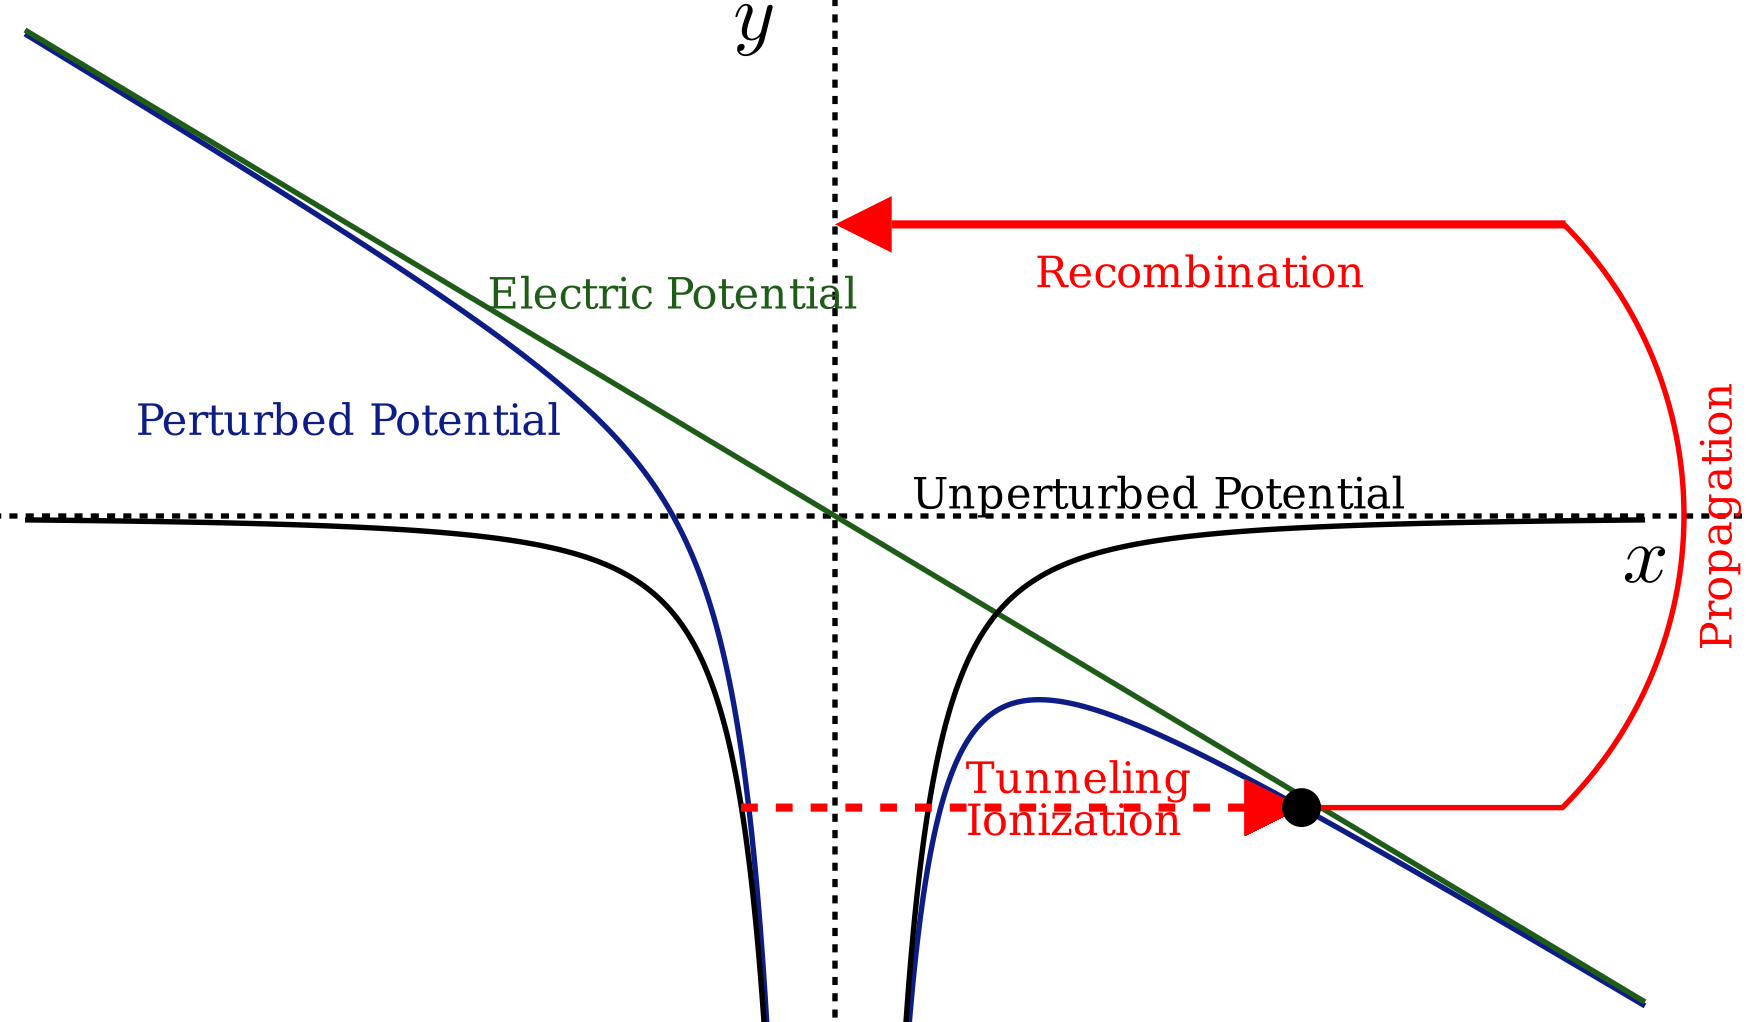
\includegraphics[width=0.95\textwidth]{images/three_step_one.png}
%     % \caption{The Three Step Model}
%     \label{fig:3-step-1}
% \end{minipage}
% \begin{minipage}{0.45\textwidth}\raggedleft
%     % \centering
%     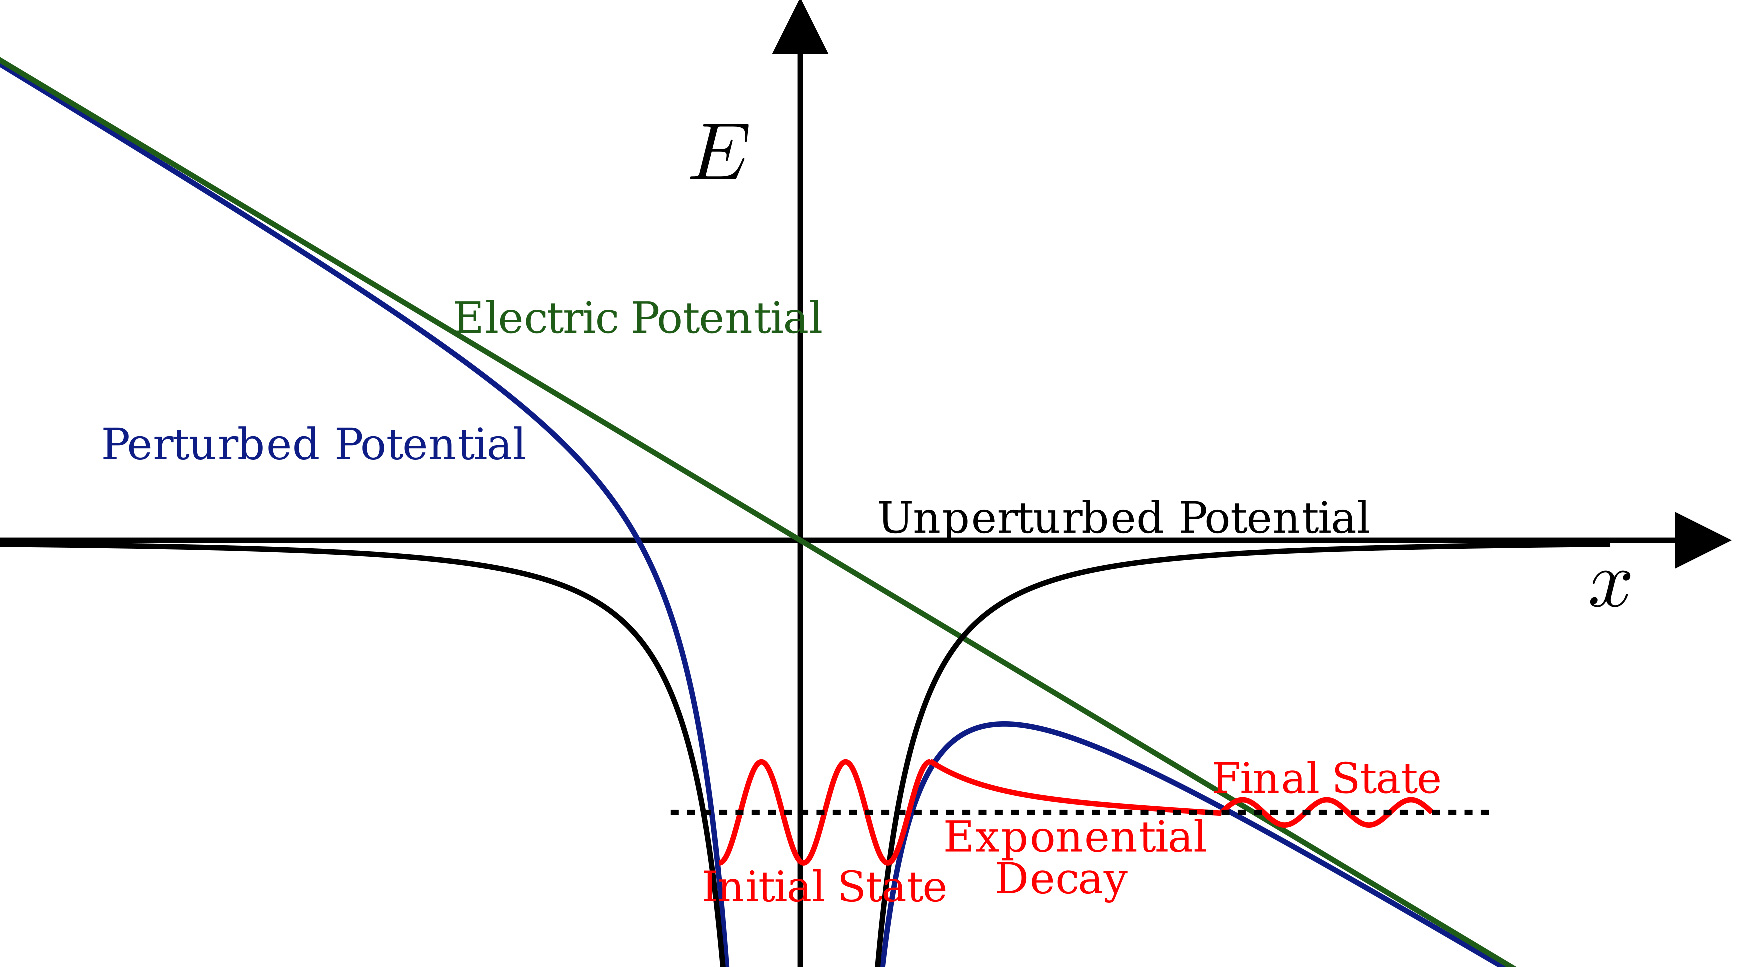
\includegraphics[width=0.95\textwidth]{images/three_step_two.png}
%     % \caption{The Three Step Model}
%     \label{fig:3-step-2}
% \end{minipage}
\begin{figure}[h]
    \centering
    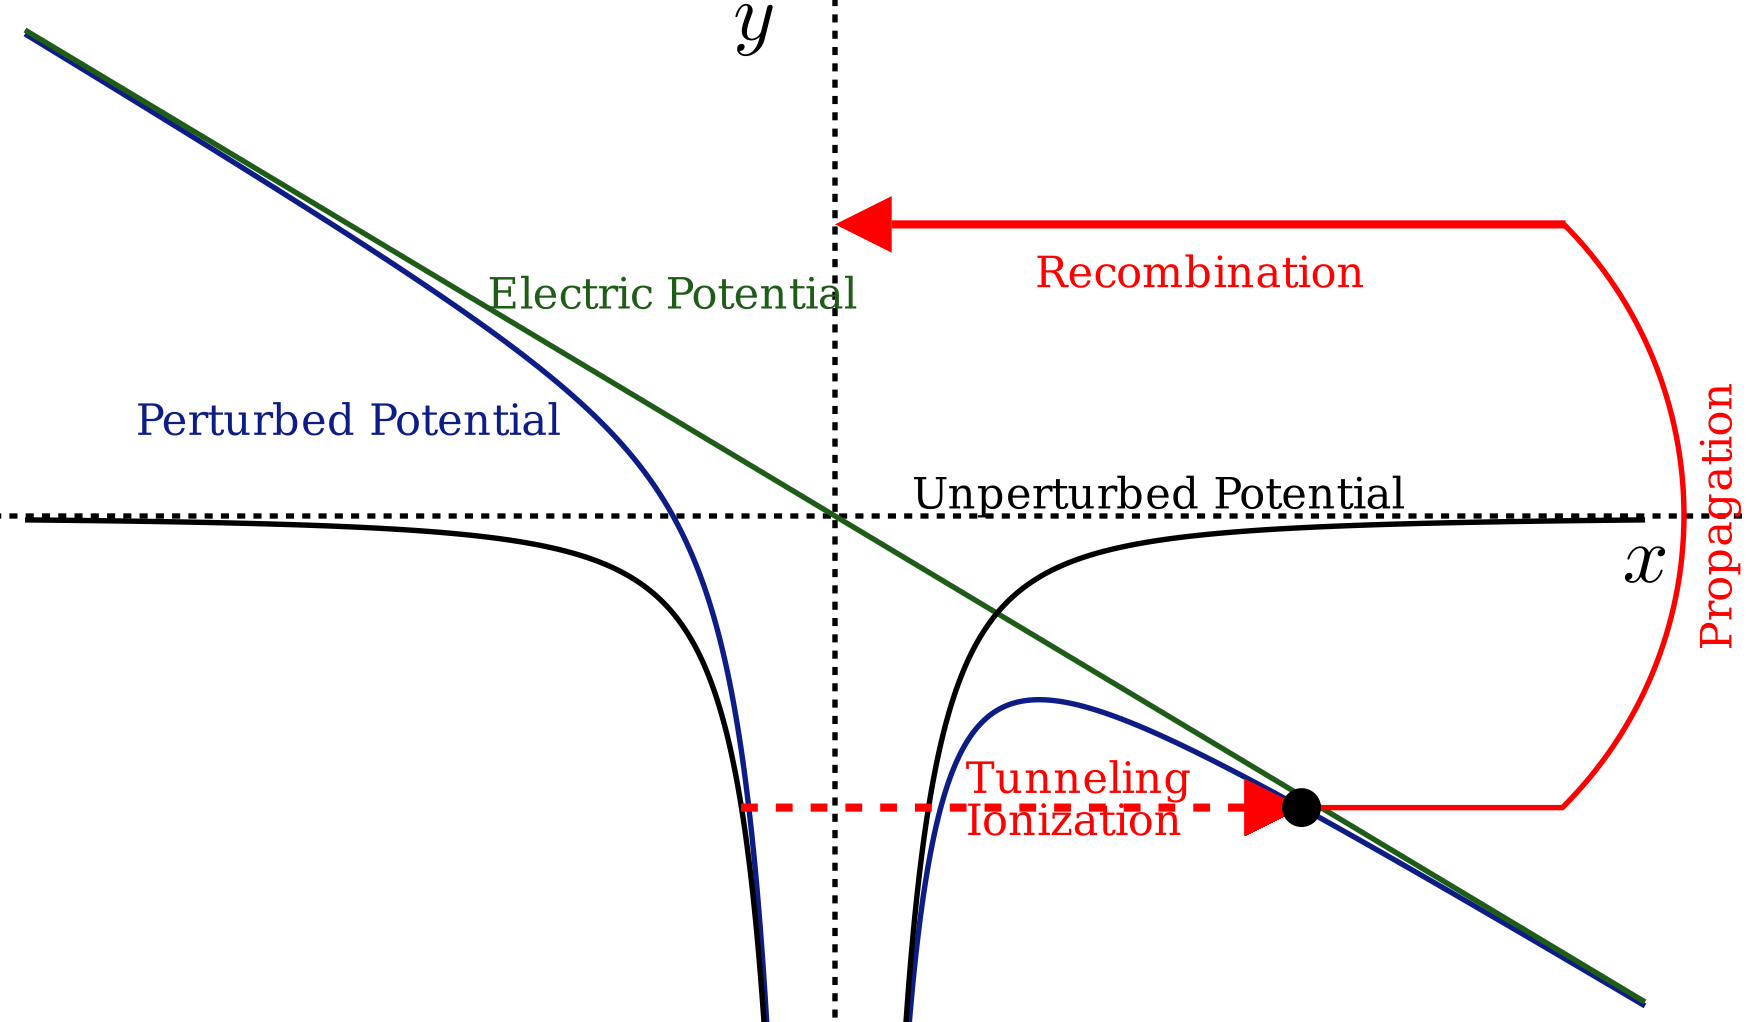
\includegraphics[width=0.8\textwidth]{images/three_step_one.png}
    \caption{The Three Step Model}
    \label{fig:3-step-1}
\end{figure}

\begin{figure}[h]
    \centering
    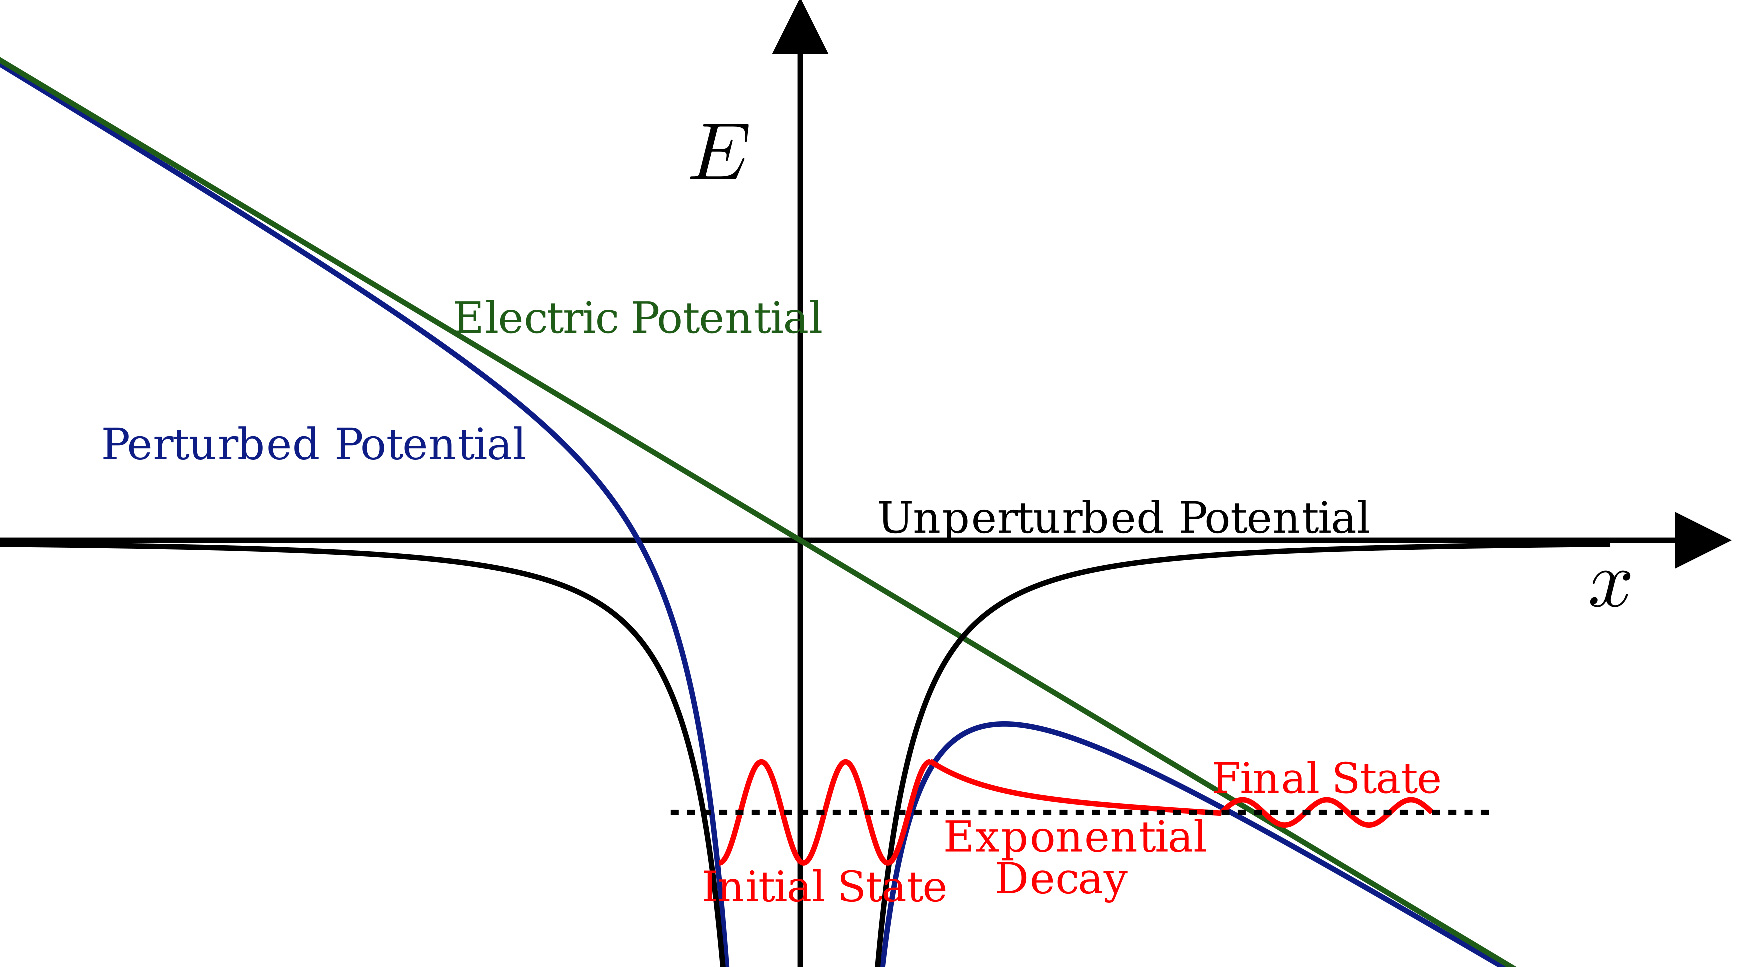
\includegraphics[width=0.8\textwidth]{images/three_step_two.png}
    \caption{The Three Step Model}
    \label{fig:3-step-2}
\end{figure}

\subsection{HHG in Plasma}
The spectrum from HHG consists of a number of integer harmonics of the incident laser pulse (with their intensities decreasing), followed by a plateau where the harmonic intensity is nearly constant over many orders and a sharp cutoff. A number of models and theories have been proposed explaining this power law and cutoff.

Bezzerides et al. \cite{hhg-relativistic} gave the first model way back in 1983. Their model was based on relativistic equation of motion and hydrodynamics approxiamation. They found out a cutoff frequency as
\begin{equation}
    \label{eq:cutoff-relativistic}
    n_{\max}^2 = n_p/n_c
\end{equation}
where $n_p$ is the plasma density and $n_c$ is the critical density. They demonstrated that the principal source of high-harmonic emission is the strong non linear restoring force which exists when resonant absorption occurs in a highly steep density profile. However, this model was not able to explain the plateau region as well as the fact that we get harmonics which are much higher that the cutoff frequency given by Eq. \ref{eq:cutoff-relativistic}.

\subsection{Oscillating Mirror Model}
To induce large intensity boosts on the reflected laser beam, plasma mirrors need to be set in relativistic motion, which is possible when they are exposed to laser intensities ranging from at least $10^{18} W/cm^2$ up to the highest laser intensities available to date, of a few $10^{22} W/cm^2$. The incident laser field then drives a periodic oscillation of the plasma mirror surface, at relativistic velocities. This relativistic oscillating mirror induces a periodic Doppler effect on the reflected field. Each time the mirror surface moves outward, it compresses the laser energy in time, leading to a sharpening of the reflected waveform. Although still periodic in time, this waveform is no longer sinusoidal: its spectrum thus consists of the combination of the laser frequency $\omega_p$ with a comb of high-order harmonics of frequencies $n\omega_p$.

The model assumes that the duration of the light pulse is sufficiently short so that the motion of the ions may be neglected. The ions are treated as a fixed positive background charge. Also, the model neglect the details of the changes of the electron density profile and to represent the collective electronic motion by the motion of the boundary of the supercritical region. This boundary represents an effective reflecting surface performing an oscillatory motion, the oscillating mirror. Using these assumptions, we follow von der Linde et al. \cite{hhg-main} to derive th spectrum of HHG. First, we show that the HHG can be understood as a phase modulation due to the moving mirror.

For this, neglecting for a moment retardation effects the phase shift of the reflected wave resulting from a sinusoidal displacement of the reflecting surface in the z-direction:

\begin{equation*}
    s(t) = s_0 \sin(\omega t)
\end{equation*}

is given by
\begin{equation*}
    \phi(t) = (2\omega_0s_0/c)\cos\alpha \sin \omega_m t
\end{equation*}

where $\alpha$ is the angle of incidence and $\omega_m$ is the mirror frequency (modulation frequency). The electric field of the reflected wave is given by

\begin{equation}
    E_R \propto e^{-i\omega_0 t}e^{i\phi(t)} =  e^{-i\omega_0 t} \sum _{n \to -\infty}^{n \to -\infty}J_n(\chi) e^{-in\omega_m t}
\end{equation}

where $J_n(\xi)$ is the Bessel function of order $n$ and
\begin{equation}
    \label{eq:chi-def}
    \chi = \frac{2\omega_0s_0\cos\alpha}{c}
\end{equation}

This shows that the phase modulation produced by the oscillating mirror gives rise to a series of sidebands at distances from the carrier frequency $\omega_0$ given by multiples of the modulation frequency $\omega_m$.

The reflecting surface performs a periodic motion at a frequency $2\omega_0$, or a superposition of $\omega_0$ and $2\omega_0$ , depending on the polarization and angle of incidence of the incoming light. Thus, the modulation frequencies provided by the mirror motion are $\omega_m = \omega_0$ and/or $\omega_m = 2\omega_0$. The key point is that this type of modulation produces sidebands representing even and odd harmonics of the fundamental frequency $\omega_0$ . These ideas suggests an interpretation of high-order harmonic generation from a plasma-vacuum interface as a phase modulation from a periodically moving reflecting surface.

\subsubsection{s- and p-Polarization}

\begin{itemize}
    \item \textbf{p-Polarized Light}: The electric and the magnetic field are, respectively, parallel and perpendicular to the plane of incidence. The electrons move in the plane of incidence. The electron boundary is driven at frequencies $\omega_0$ and $2\omega_0$ , because both the transverse and the longitudinal component of the electron velocity contribute to the motion of the boundary. It follows that in this case both even and odd harmonics with p-polarization are generated. See Fig. \ref{fig:p-polarized}.
          \begin{figure}[h]
              \centering
              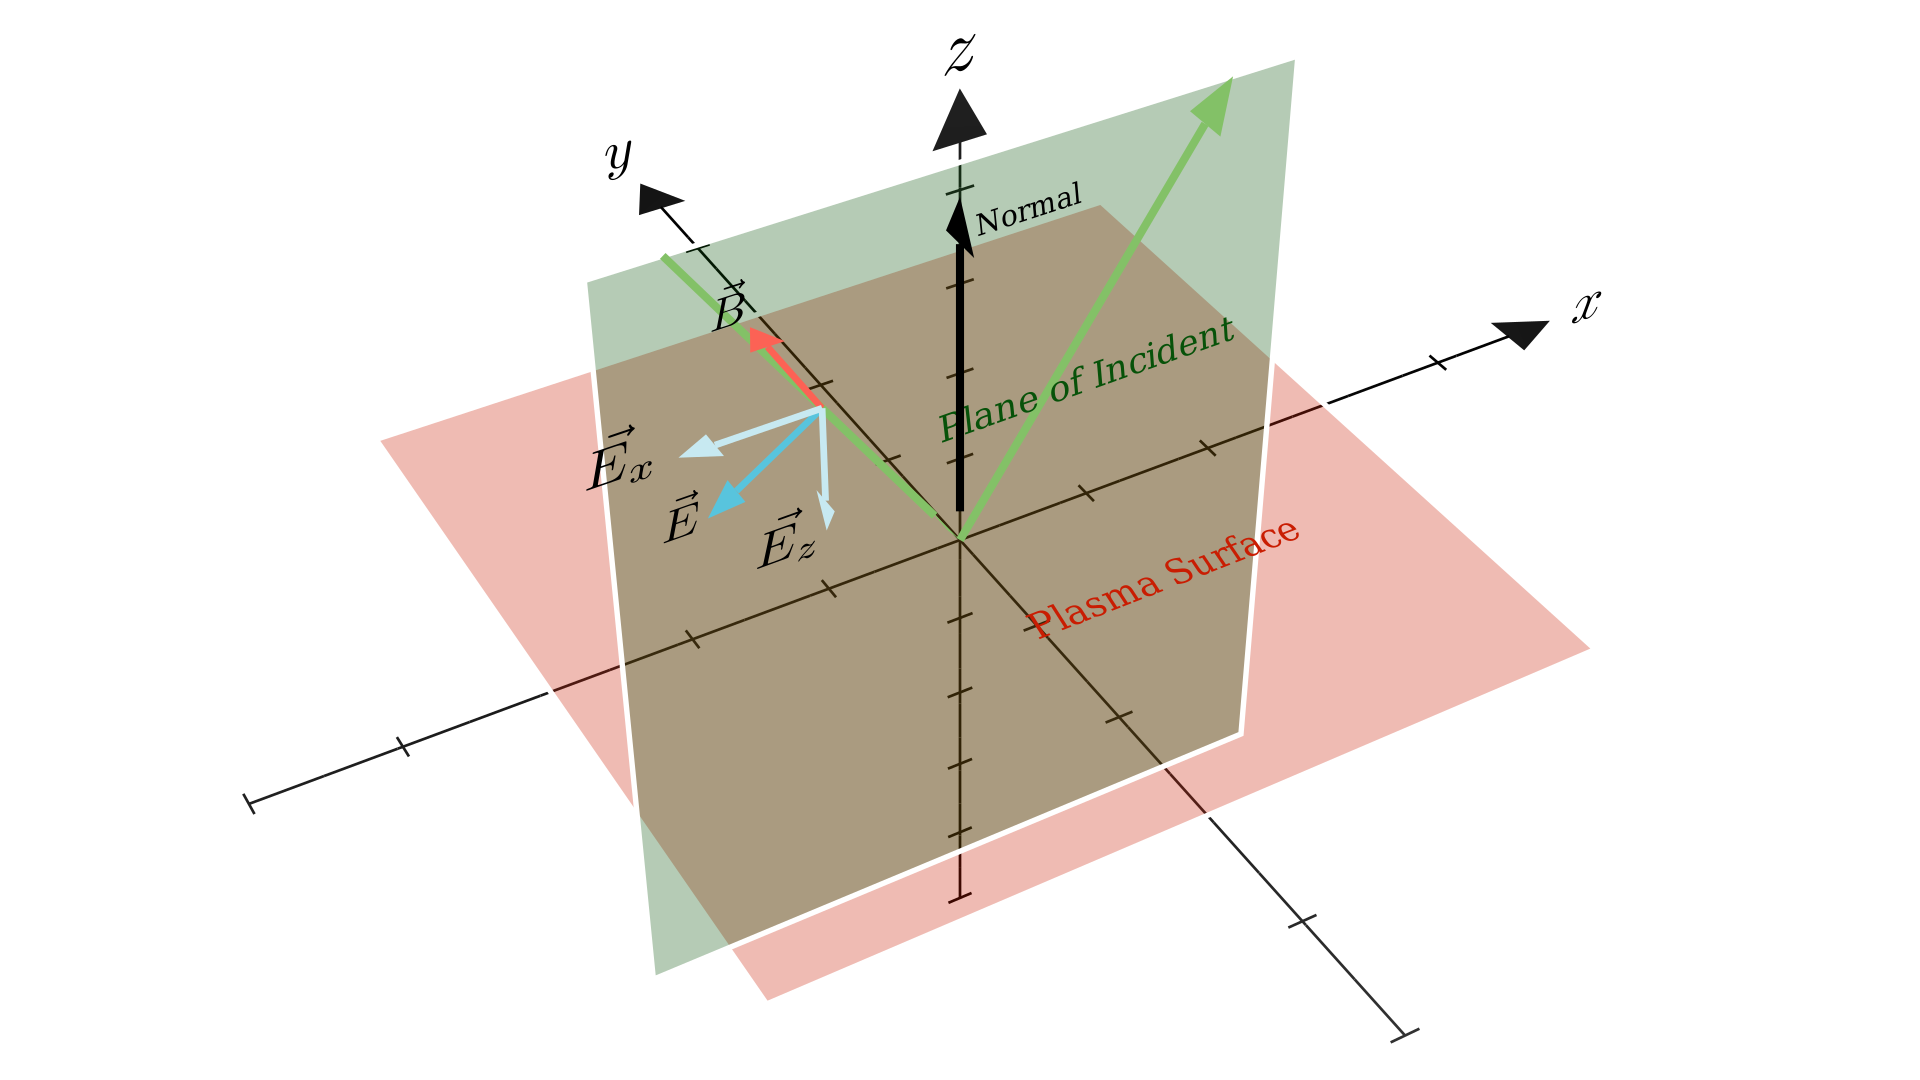
\includegraphics[width=1\textwidth]{images/p.png}
              \caption{The electric and magnetic field of the incident light are, respectively, parallel and perpendicular to the plane of incidence. The electrons move in the plane of incidence.}
              \label{fig:p-polarized}
          \end{figure}

    \item \textbf{s-Polarized Light}: The electric field is parallel to the plasma—vacuum interface. The electrons move in a plane perpendicular to the plane of incidence. In this configuration only the longitudinal component contributes, while the transverse component of the electron motion is ineffective. The normal motion of the mirror is driven at one frequency only, $\omega_m = 2\omega_0$. It follows that the reflected light is composed of s-polarized odd harmonics and p-polarized even harmonics. See Fig. \ref{fig:s-polarized}.
          \begin{figure}[h]
              \centering
              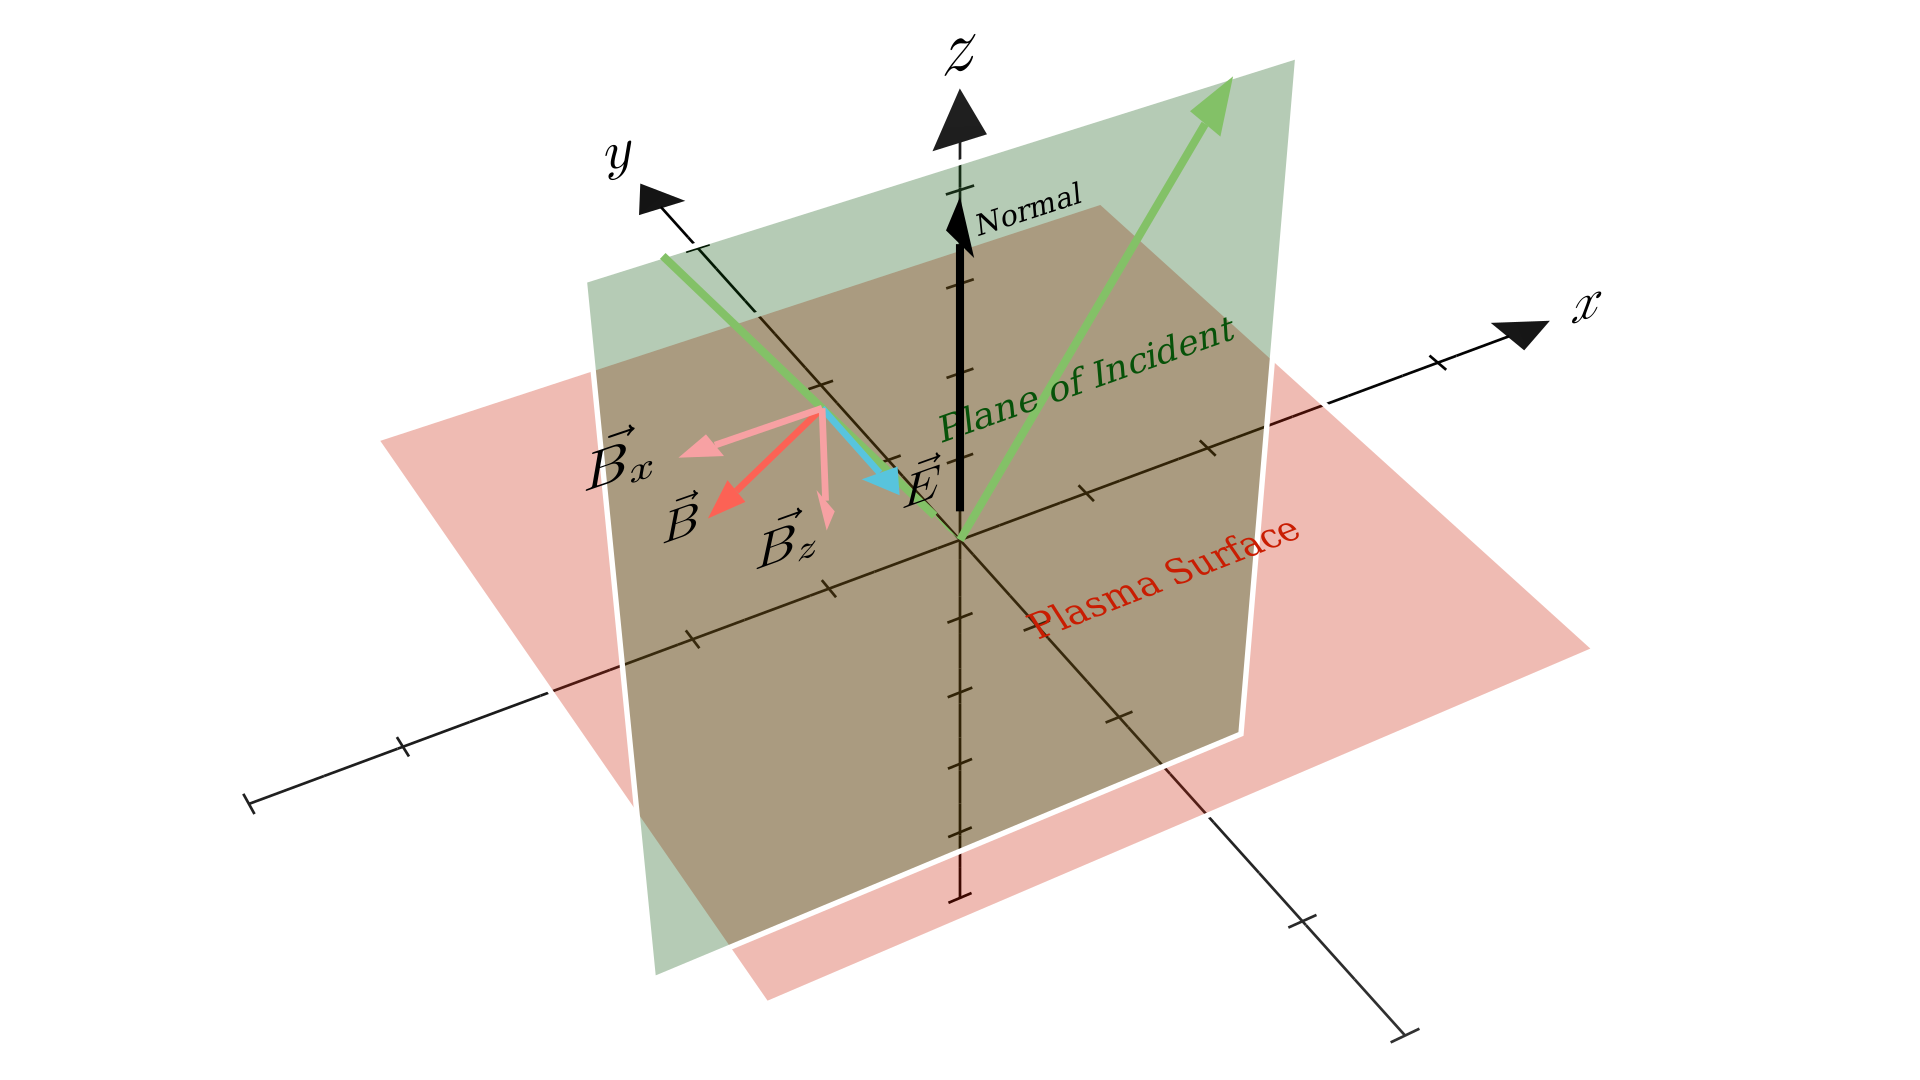
\includegraphics[width=1\textwidth]{images/s.png}
              \caption{The electric field of the incident light is parallel to the plane of incidence. The electrons move in a plane perpendicular to the plane of incidence.}
              \label{fig:s-polarized}
          \end{figure}
\end{itemize}
\begin{table}[h]
    \caption{Polarization Selection Rule}
    \vspace{0.5cm}
    \label{tab:selection-rule}
    \begin{tabular}{|l|l|l|}
        \hline
                                         & \textbf{s-polarized Harmonics} & \textbf{p-polarized Harmonics} \\ \hline
        \textbf{s-Polarized Fundamental} & Odd                            & Even                           \\ \hline
        \textbf{p-Polarized Fundamental} & None                           & Odd and Even                   \\ \hline
    \end{tabular}
\end{table}

\subsubsection{HHG Spectrum}
We chose the coordinate system shown in Fig. \ref{fig:s-polarized}. The incident light is polarized along the $y$-axis. The electric field of the incident light is given by:
\begin{equation*}
    E(t, x, z) = E_0 \exp\left(-i\omega_0\left(t-x/c \sin\alpha - z/c \cos\alpha\right)\right)
\end{equation*}

We assume the surface oscillations to be of the form:
\begin{equation*}
    s(t) = s_0 \sin\left( \omega_m \left(t - x/c \sin\alpha\right) \right)
\end{equation*}

The maximum displacement of the surface is $s_0$ is limited by the condition that the velocity must not exceed the speed of light. For example, for s-polarization, as $\omega_m = 2 \omega_0$, we have
\begin{align*}
    s_0 < \frac{c}{\omega_0} & = \frac{c}{2\omega_0} \\
    \therefore \chi          & < \cos\alpha
\end{align*}

We assume that the reflected wave can be written in the general form of a plane wave propagating in the specular direction:

\begin{equation*}
    E_R = G(u) = G(t - x/\sin\alpha + z/\cos\alpha)
\end{equation*}

If we further assume that the surface is completely reflecting, then $G(u)$ is obtained from the condition that the total field must vanish on the reflecting surface $z = s(t,x)$, that is:
\begin{equation}
    \label{eq:bc}
    E(t,x,s(t,x)) + E_R(t,x,s(t,x)) = 0
\end{equation}

Both sides of Eq. \ref{eq:bc} are a function only of $\xi = t - x/c \sin\alpha$. The spectrum of the reflected wave can be determined using the Fourier transform of $G(u)$:
\begin{equation*}
    G(\omega) = \int_{-\infty}^{\infty} G(u) e^{-i\omega u} du
\end{equation*}

where $u = \xi - s_0/c \cos\alpha \sin(\omega_m \xi)$ Integrating, this comes out to be:
\begin{equation}
    \label{eq:G_omega}
    G(\omega) = -2 \pi E_0 \sum_{-\infty}^{+\infty} \frac{1}{1+ n\omega_m /2 \omega_0} \times J_n \left(\left( 1+ n\omega_m /2\omega_0\right)\xi\right)\delta \left(\omega - \omega_0 - n\omega_m\right)
\end{equation}

where $J_n$ are the Bessel functions of order n.

For a s-polarization we have, $\omega_m = 2 \omega_0$ and hence equation \ref{eq:G_omega} reduces to:
\begin{equation}
    \label{eq:s-spectrum}
    S((2n+1)\omega_0) = (\pi E_0)^2\left(\frac{J_n((n+1)\xi)}{(n+1)}- \frac{J_{n+1}(n\xi)}{(n)}\right)^2
\end{equation}

For a p-polarization:
\begin{equation}
    \label{eq:p-spectrum}
    S(n\omega_0) = (\pi E_0)^2\left(\frac{J_{n-1}(\frac{1}{2}(n+1)\xi)}{\frac{1}{2}(n+1)}- \frac{J_{n+1}\frac{1}{2}((n-1)\xi)}{\frac{1}{2}(n-1)}\right)^2
\end{equation}

A plot of the spectra is shown in the figure \ref{fig:spectrum}
\begin{figure}[h]
    \centering
    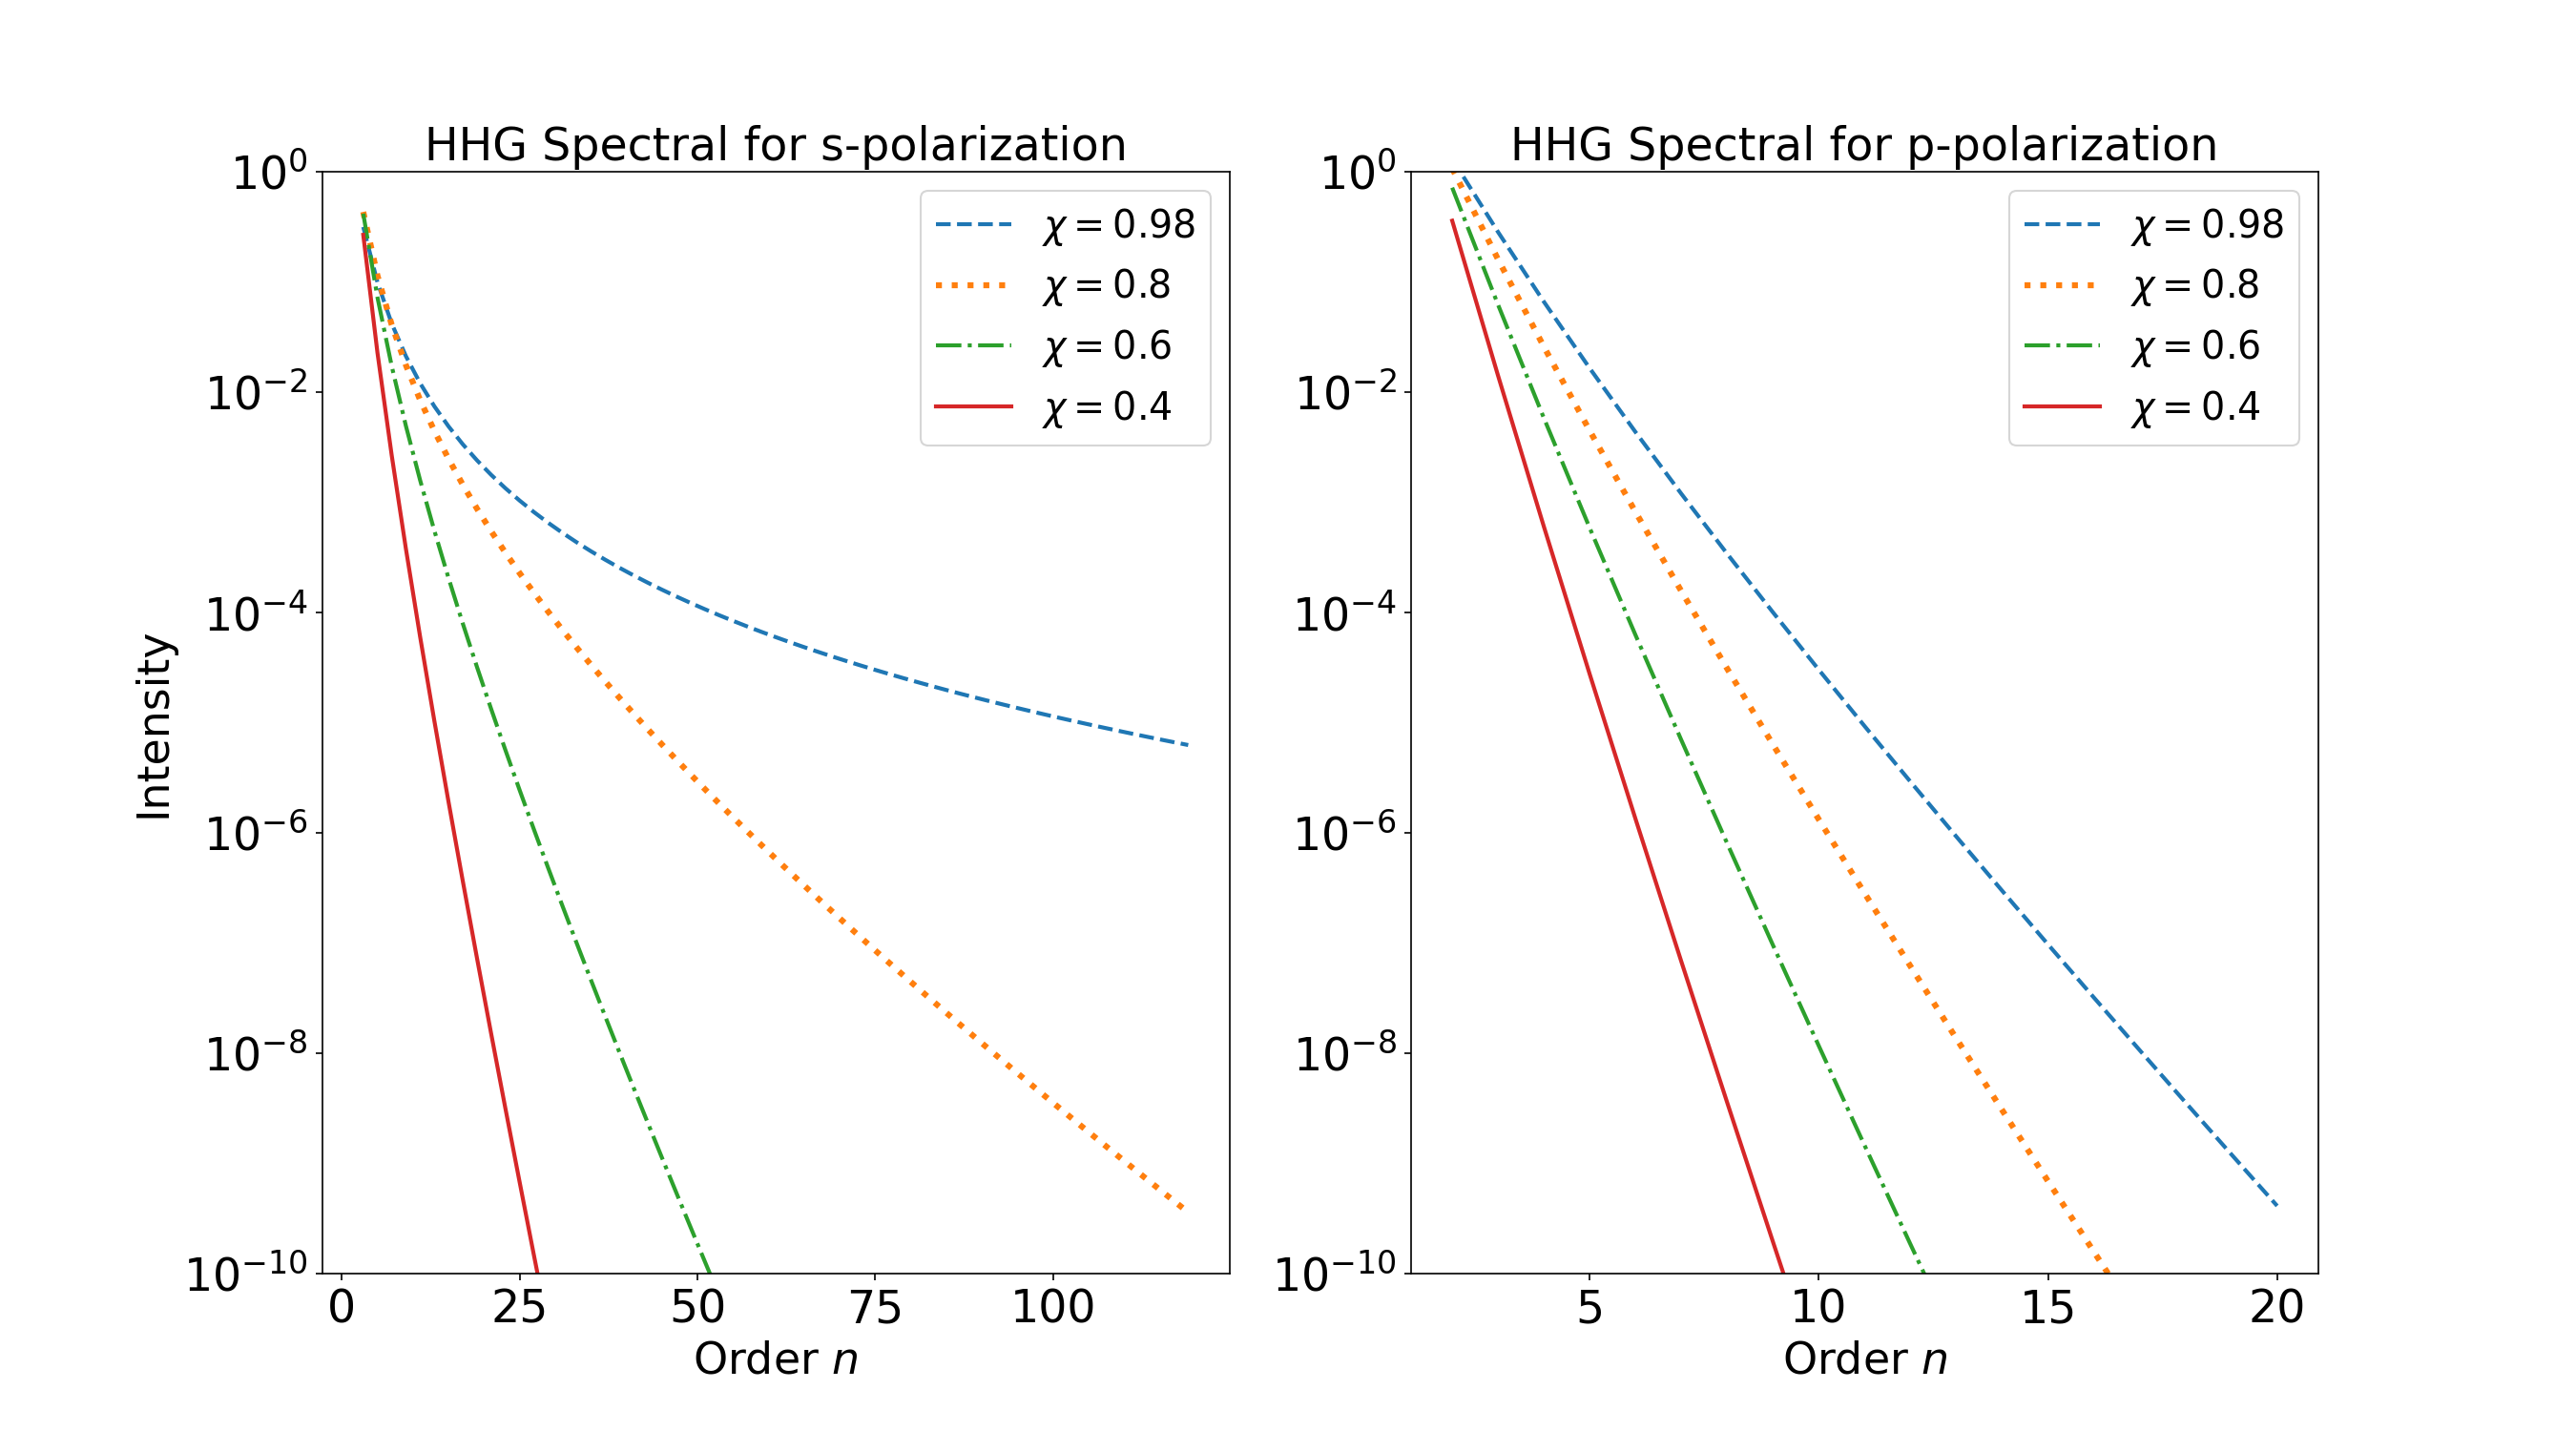
\includegraphics[width=1\textwidth]{images/spectrum.png}
    \caption{HHG spectrum for s and p polarization. The amplitudes of HHG is decreasing more rapidly for p-polarization that s-polarization}
    \label{fig:spectrum}
\end{figure}
\subsection{Universal Spectra}
The \textit{ideal mirror} assumptions made by von der Linde et al.\cite{hhg-main} are not held in practice. In fact, ideal mirror is not physically possible. Gordienko et al.\cite{universal-spectra} showed that it is not necessary to assume a form of plasma surface oscillation if the goal is just to get the cutoff and power law of the HHG spectrum. Assuming only the boundary condition equation \ref{eq:bc} and the periodicity of the surface motion, they found the following results which is valid for any type of plasma surface motion:
\begin{enumerate}
    \item The power law for monochromatic wave
          \begin{equation}
              \label{eq:power-law-u}
              I_n \propto 1/n^{5/2}
          \end{equation}
    \item The power law for broadband wave
          \begin{equation*}
              I_n \propto 1/n^{5/2}
          \end{equation*}
    \item The cutoff
          \begin{equation}
              \label{eq:cutoff-u}
              n_c \propto 4\gamma_{\max}^2
          \end{equation}
\end{enumerate}

\subsection{Simulation Setup}
Simulations are performed using \textit{EPOCH}\cite{EPOCH}. The simulation setup is consist of some experiments done using normal incidence while other experiments are done with oblique incidence.
\subsubsection{For Normal Incident}
The simulation box extends for $40 \lambda _l$ (from $-20 \lambda _l$ to $20 \lambda _l$), where $\lambda_l$ is the laser wavelength taken as $1\mu m$ and has total 16000 cells, i.e., 400 cells per wavelength. The plasma is placed at $x=0$ and with a thickess of $\lambda_l$. Number of particles per cell are 100. The pulse duration is $T = 20 \tau$ and simulation is run till $T_{end} = 40 \tau$. Here $\tau$ is the time period of laser pulse. The study of SG envelope is perfomed in the normal incidence. So, the envelope used is SG given by:
\begin{equation}
    \label{eq:sg}
    P = P_0 \exp\left( -2 \left(\frac{x - \mu}{\sigma}\right)^p\right)
\end{equation}
where $P_0$ is the normalization constant, $\mu$ is the mean, $\sigma$ is the standard deviation and $p$ is the power of the SG.

\subsubsection{For Oblique Incident}

To article uses only a 1d simulation for oblique incidence. This is accomodated by following Bourdier \cite{2d-transformation} transformation, where simulations are perfomred in a moving frame in which the light is normally incident. (See the figure \ref{fig:frames})

\begin{figure}[h]
    \centering
    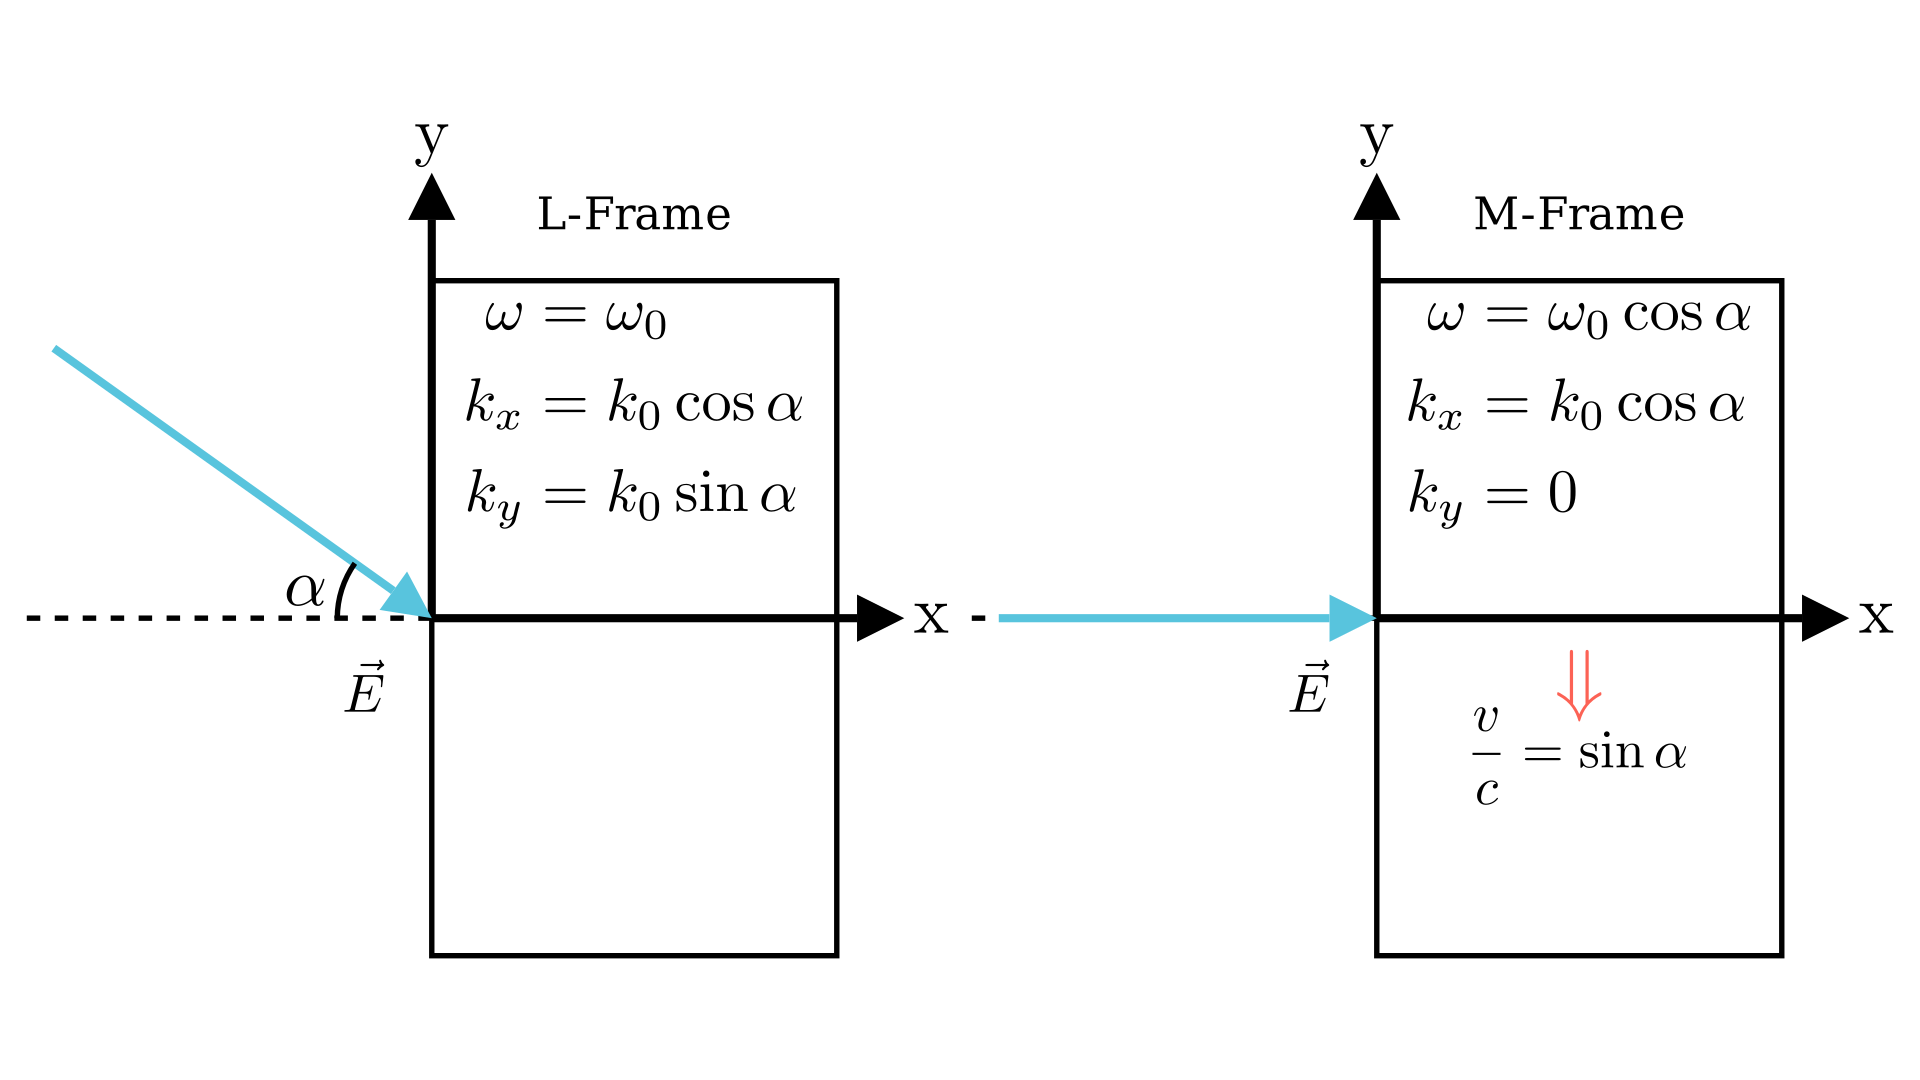
\includegraphics[width=1\textwidth]{images/frames.png}
    \caption{L is the lab frame and M is the moving frame. Simulations are done in M-frame and then they are transformed back to the L-Frame}
    \label{fig:frames}
\end{figure}

To do this, we make a Lorentz transformation from the laboratory frame L to a frame M, moving in y direction with a velocity of $\mathbf{v_M} = c\sin\alpha \hat{y}$. This way, the incident pulse is normal to the surface in the M-frame as the figure shows. This makes the plasma to move with a velocity of $-\mathbf{v_f}$. The frequency $\omega_0$ and the wave vector $\mathbf{k}_0$ changes so that the speed of light is the same. The transformations of these are:
\begin{align}
    \label{fig:omega-k}
    \begin{split}
        \omega_L     & = \omega_0                                      \\
        \omega_M     & = \omega_0\cos\alpha                            \\
        \mathbf{k}_L & = k_0\cos\alpha \hat{x} + k_0\sin\alpha \hat{y} \\
        \mathbf{k}_M & = k_0\cos\alpha \hat{x}
    \end{split}
\end{align}

The electric and magnetic field also changes. For p-polarization:

\begin{align}
    \label{eq:field-p}
    \begin{split}
        \mathbf{E}_L  & = E_0(-\sin\alpha \hat{x} + \cos\alpha \hat{y}) \\
        \mathbf{E}_M  & = E_0\cos\alpha \hat{y}                         \\
        c\mathbf{B}_L & = E_0\hat{z}                                    \\
        c\mathbf{B}_M & = E_0\cos\alpha \hat{z}
    \end{split}
\end{align}

While, for s-polarization:

\begin{align}
    \label{eq:field-s}
    \begin{split}
        \mathbf{E}_L & = E_0\hat{z}                                    \\
        \mathbf{E}_M & = E_0\cos\alpha \hat{z}                        \\
        c\mathbf{B}_L & = E_0(\sin\alpha \hat{x} - \cos\alpha \hat{y}) \\
        c\mathbf{B}_M & = -E_0\cos\alpha \hat{y}
    \end{split}
\end{align}

Note that the fiels amplitudes ar decreased by a factor of $\cos\alpha$ and hence intensity also decreases. However, the normalized vector potential $a_0 = eE_0/m\omega_0c$ remains invariant. The density becomes $n_M = n_0/\cos\alpha$. A summary of these transformations is given in the table below:
\begin{table}[!ht]
    \centering
    \caption{Transformation Equations}
    \label{tab:transformation}
    \vspace{0.3cm}
    \begin{tabular}{|l|l|l|}
        \hline
        \textbf{Quantity}          & \textbf{L-Frame}                                 & \textbf{M-Frame}          \\ \hline
        $\omega$                   & $\omega_0$                                       & $\omega_0 \cos\alpha$     \\ \hline
        $\lambda$                  & $\lambda_0$                                      & $\lambda_0/\cos\alpha$    \\ \hline
        $n$                        & $n_0$                                            & $n_0/\cos\alpha$          \\ \hline
        $\mathbf{E}$ (p-polarized) & $E_0 (-\sin\alpha \hat{x} + \cos\alpha \hat{y})$ & $E_0 \cos\alpha \hat{y}$  \\ \hline
        $\mathbf{E}$ (s-polarized) & $E_0 \hat{z}$                                    & $E_0 \cos\alpha \hat{z}$  \\ \hline
        $\mathbf{B}$ (p-polarized) & $E_0 \hat{z}$                                    & $E_0 \cos\alpha \hat{z}$  \\ \hline
        $\mathbf{B}$ (s-polarized) & $E_0 (\sin\alpha \hat{x} - \cos\alpha \hat{y})$  & $-E_0 \cos\alpha \hat{y}$ \\ \hline
    \end{tabular}
\end{table}

\section{Summary of Work Done in Previous Semester}
Here is a brief summary of works done in the previous semester.

\subsection{Till Previous Semester Minor}
Our research primarily focused on studying plasma and its parameters. We then utilized the particle-in-cell algorithm to simulate the interaction between laser and both overdense and underdense plasma. Our findings revealed that the laser is reflected from overdense plasma, while underdense plasma acts as a transparent medium. We also investigated how plasma surface oscillation varies with changes in plasma density and laser intensity. Additionally, we observed that altering the laser intensity resulted in changes in the critical density for plasma.

\subsection{Till Previous Semester Major}
Following the minor presentation, our research shifted towards the study of high harmonic generation. This process involves the interaction between laser and plasma, which results in the generation of higher frequency harmonics of the incident laser radiation. To investigate this phenomenon, we performed a series of simulations, focusing on how various plasma and laser parameters affect the generated high harmonics.

Our simulations involved examining the effects of parameters such as plasma density, laser intensity, laser envelope, and laser pulse length on high harmonic generation. By systematically varying these parameters, we were able to gain a more complete understanding of the underlying physics of high harmonic generation. In particular, we were interested in understanding how the properties of the plasma affect the generation of high harmonics.

In addition to our study of plasma and laser parameters, we also extended our investigation to include the study of surface oscillation. Specifically, we aimed to understand the frequency of these oscillations and how they relate to the generation of high harmonics. Through our simulations, we found that only odd harmonics are generated in the reflected wave under normal incidence, while even harmonics are generated through the oscillation of the surface. We also observed a resonance at $n_0/n_c = 4$. We found that the envelopes had no significant effect on the outcome of our experiments.

\section{Results and Discussion}
\subsection{Super Gaussian Envelope}
The SG envelope, given by equation \ref{eq:sg} has different area for different $p$ and hence has different energy for the same given intensity. To mitigate this, the simulation is performed by multiplying the given intensity to the pulse such that the total energy of all the pulses are the same. This is done by taking a reference SG beam (we have used $p=2$), evaluating its area and then normalizing the intensities of other SG pulses by ratio of this reference area and area of the corresponding SG envelope.

\subsection{p-Polarization}
The figure \ref{fig:p-fft} shows the spectrum of HHG in L-frame, when p-polarized light is incident on the plasma. As discussed in section 2.4.1 (see that table \ref{tab:selection-rule}), the spectrum is made up of even and odd p-polarized harmonics. There are no s-polarized harmonics.
\begin{figure}[h]
    \centering
    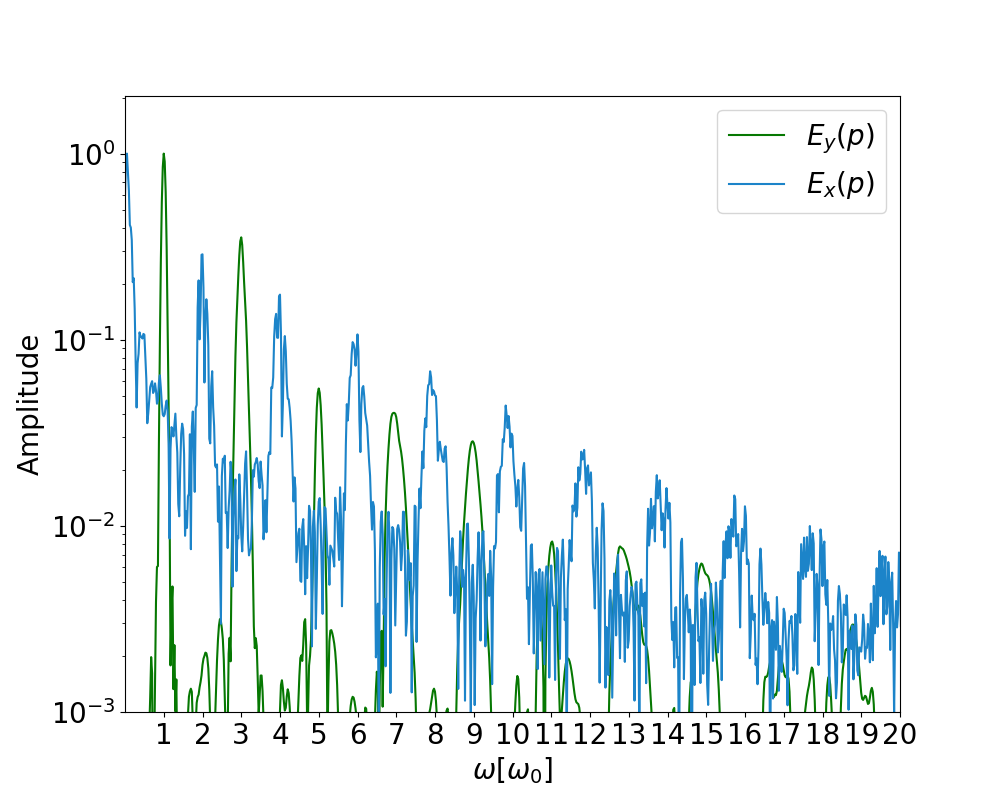
\includegraphics[width=0.8\textwidth]{images/p_fft.png}
    \caption{Spectrum of HHG for p-polarized light. Simulation parameters are $\alpha = \pi/6$, the denity is $n_0 = 7n_c$ and $a_0 = 4$}
    \label{fig:p-fft}
\end{figure}

\subsection{s-Polarization}
The L-frame spectrum of HHG is depicted in the diagram \ref{fig:s-fft}, with plasma being exposed to s-polarized light. As explained in section 2.4.1 (see that table \ref{tab:selection-rule}), the spectrum comprises of odd s-polarized harmonics and even p-polarized harmonics.
\begin{figure}[h]
    \centering
    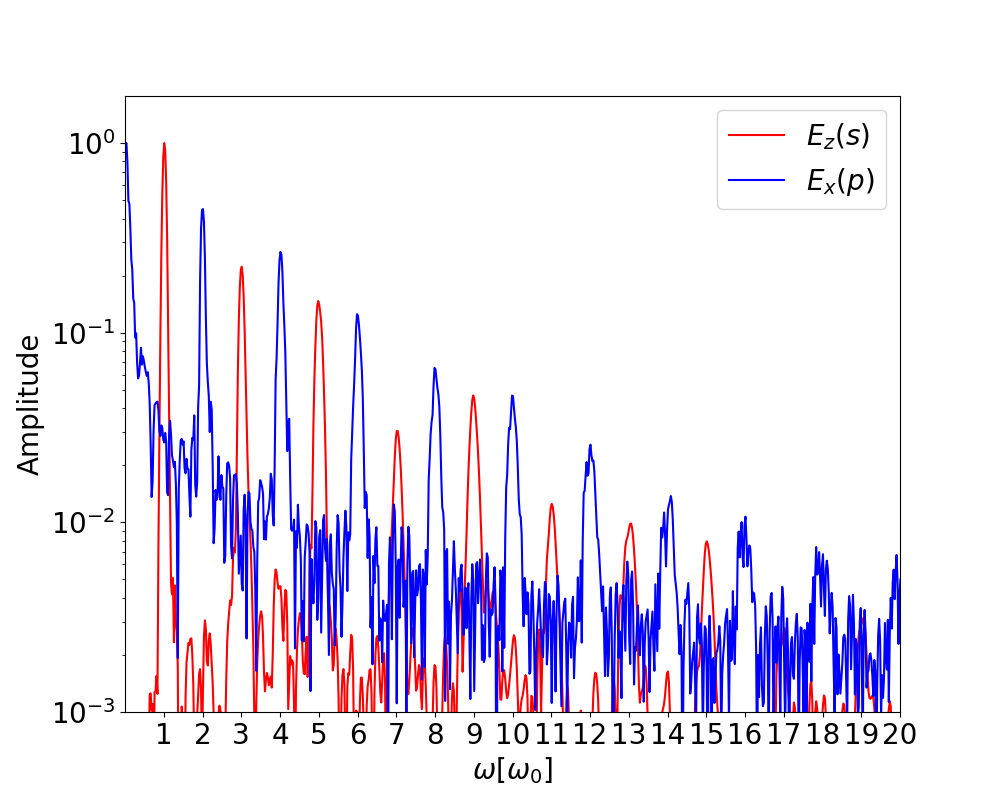
\includegraphics[width=0.8\textwidth]{images/s_fft.png}
    \caption{Spectrum of HHG for s-polarized light. Simulation parameters are $\alpha = \pi/4$, the denity is $n_0 = 7n_c$ and $a_0 = 4$}
    \label{fig:s-fft}
\end{figure}

\section{Future Plan of Work}
We plan to continue our research on high harmonic generation. Up till now, we have performed just 1D simulations. We plan to extend our simulations to 2D so that we can compare the results of oblique incident in 1D to that of 2D.

\section{Acknowledgement}
We would like to extend our sincerest gratitude to Professor Vikrant Saxena for his unwavering support, patience, motivation, enthusiasm, and invaluable guidance. His mentorship and leadership have been instrumental in the success of this project, and we feel incredibly fortunate to have had the opportunity to work with him.
% \clearpage
% \newpage
\printbibliography
% \end{changemargin}
\end{document}